\documentclass[12pt,a4paper]{report}
\usepackage{graphicx}
\usepackage{pdfpages}
\usepackage{hyperref}
\usepackage[utf8]{inputenc}
\usepackage[cyr]{aeguill}
\usepackage[francais]{babel}
\graphicspath{ {images/} }
\hypersetup{
    colorlinks,
    citecolor=black,
    filecolor=black,
    linkcolor=black,
    urlcolor=black
}
\begin{document}
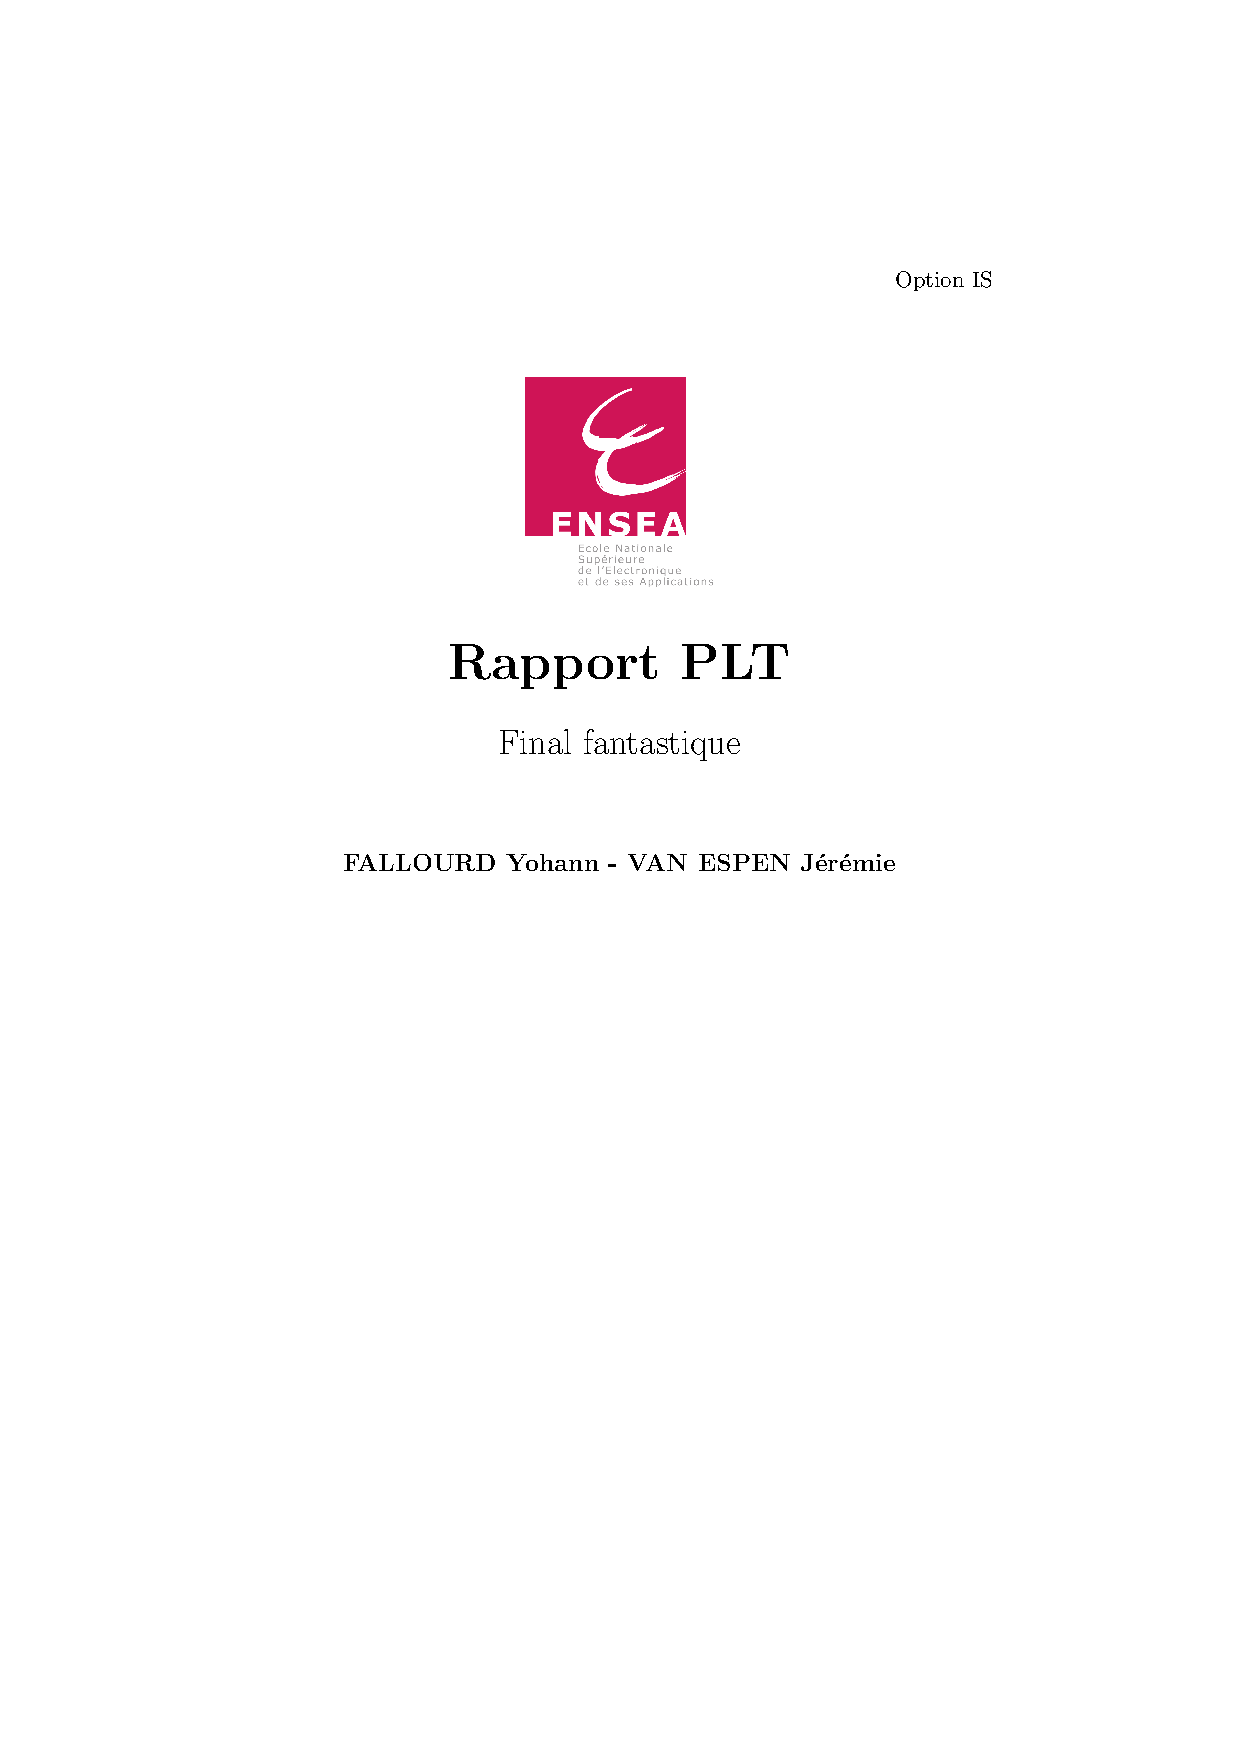
\includepdf{Titlepage}
\tableofcontents
\chapter{Objectif}
\section{Présentation générale}
Le jeu est bas\'{e} sur l'arch\'{e}type de Final Fantasy X, se distinguant par un système de combat au tour par tour ainsi que son embl\'{e}matique "sph\'{e}rier" correspondant à un arbre de talent apportant une libert\'{e} de personnalisation non n\'{e}gligeable. Voici un croquis du sphérier :

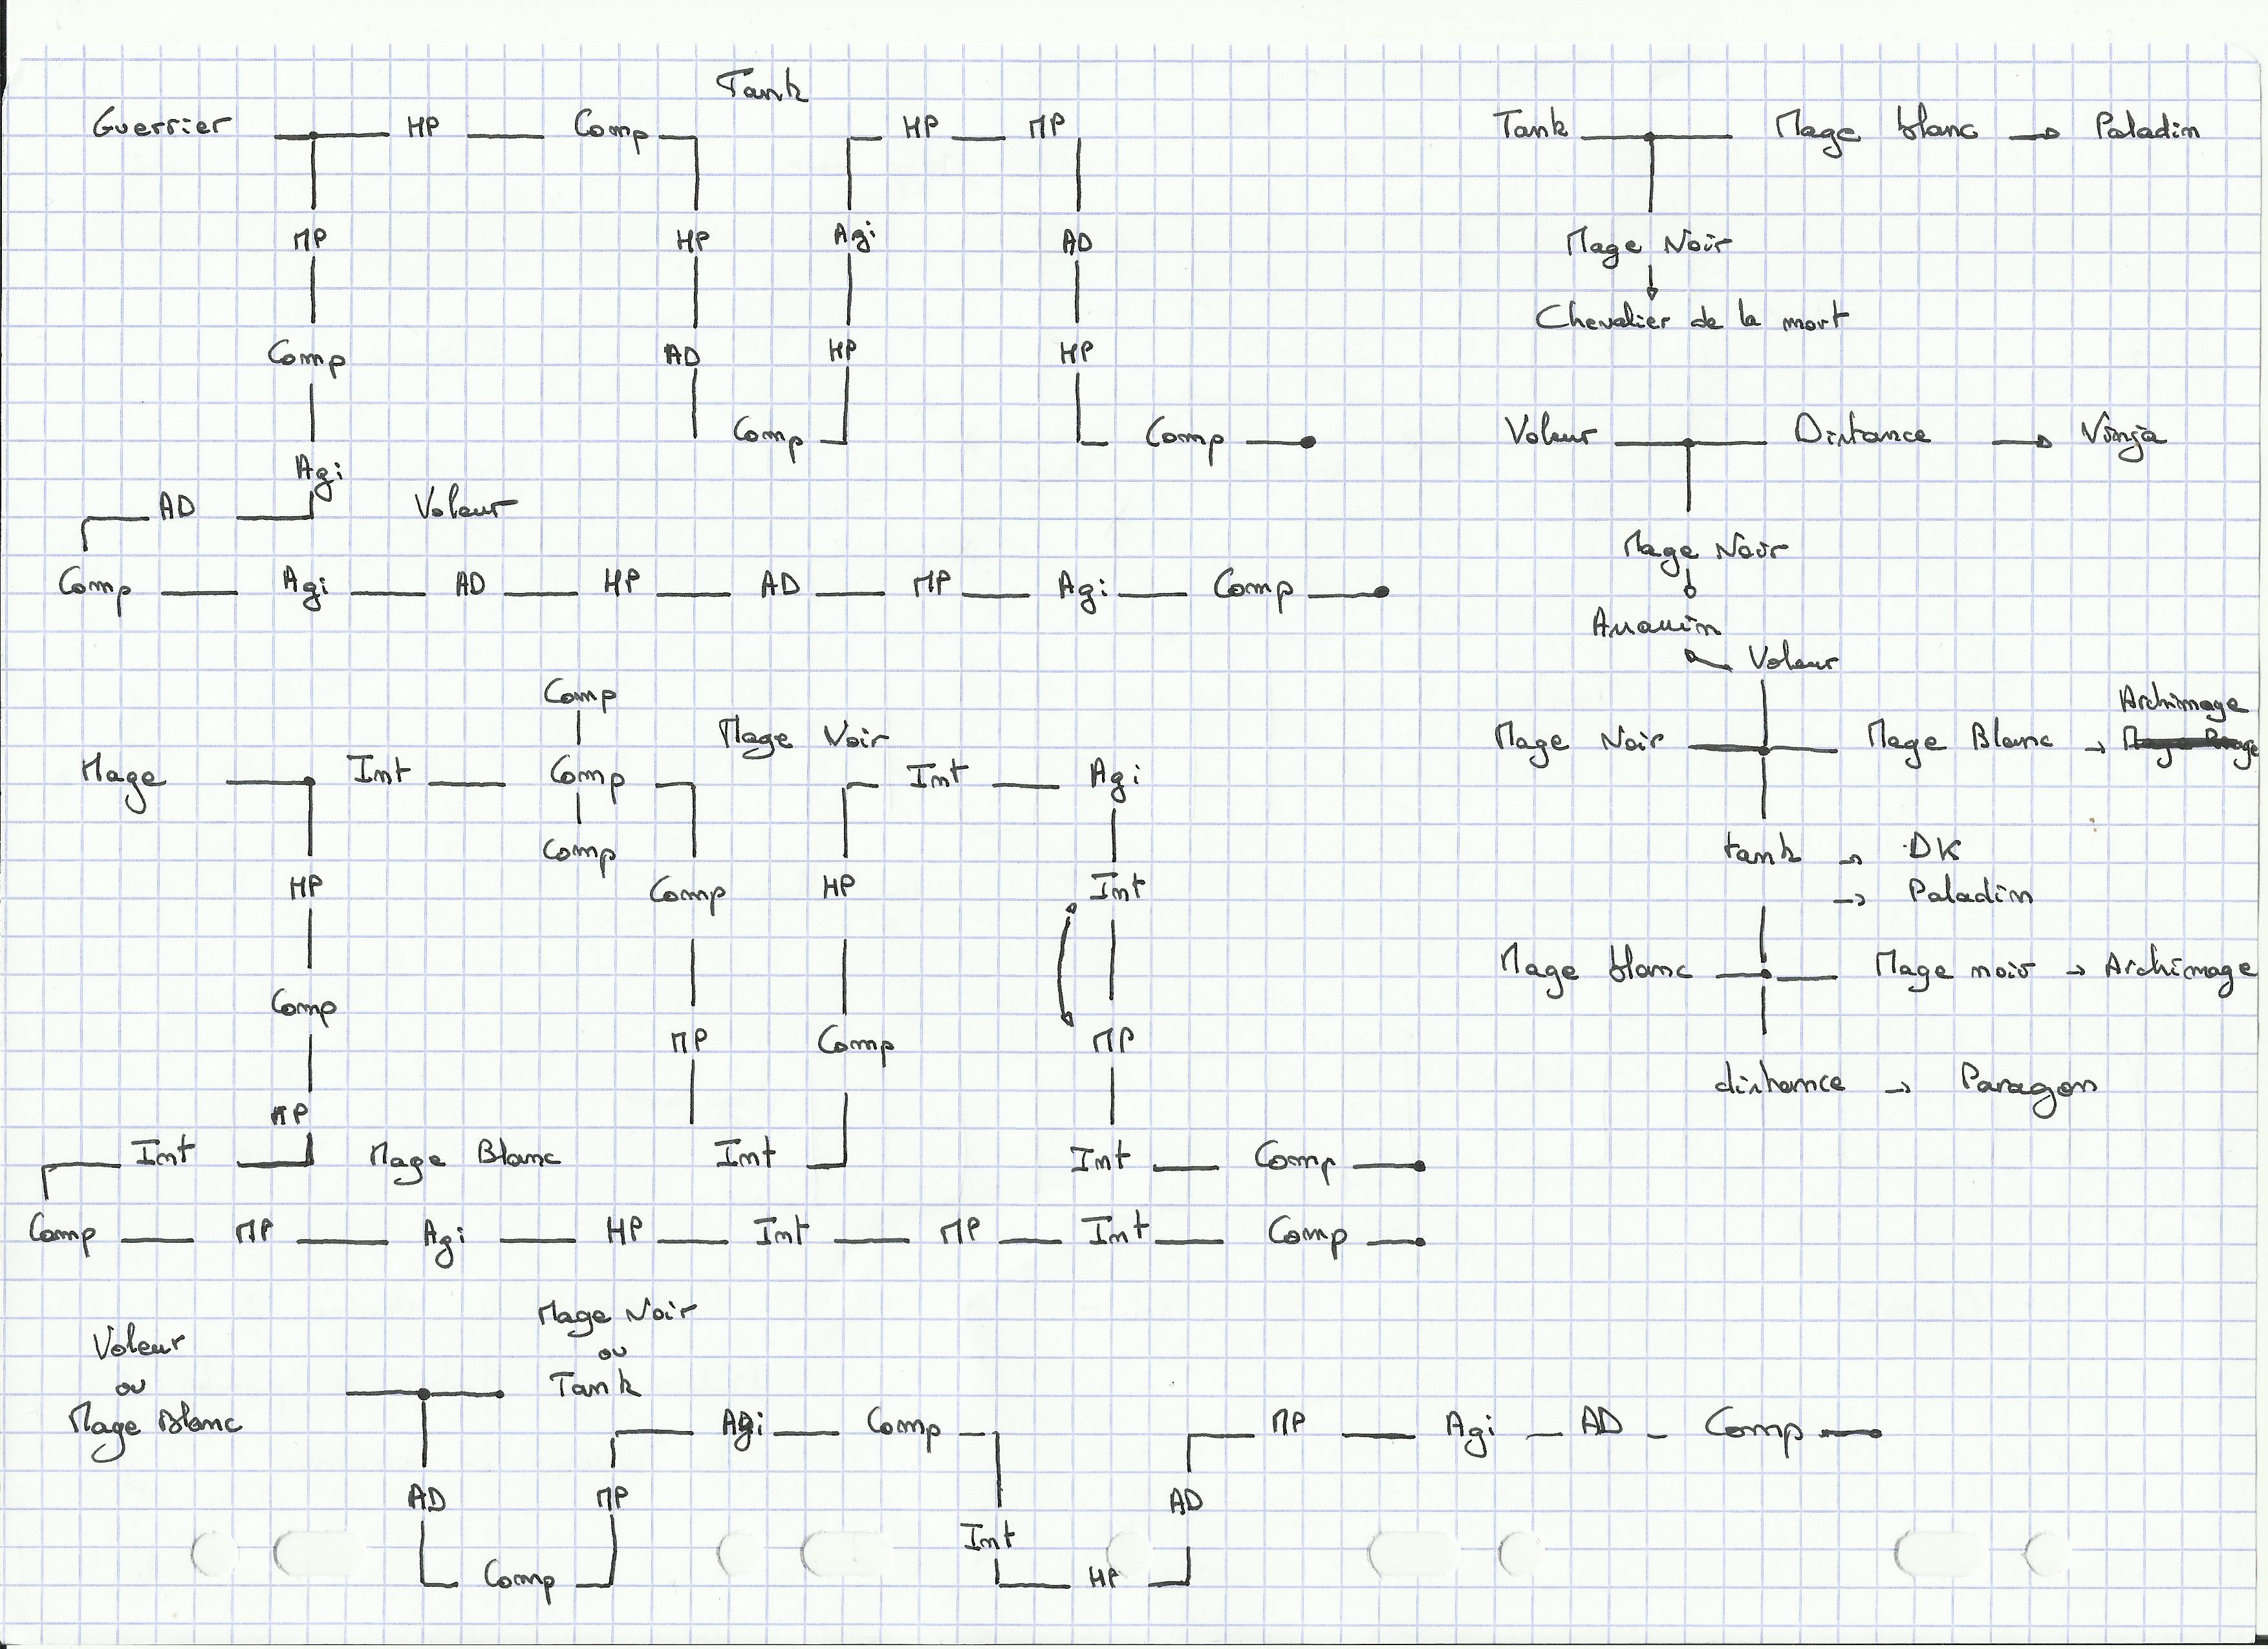
\includegraphics[width=0.80\textwidth]{Spherier.jpg}

A la diff\'{e}rence du v\'{e}ritable jeu, il n'y aura pas de d\'{e}placement libre en temps r\'{e}el; le gameplay se r\'{e}sume à un d\'{e}placement de points d'int\'{e}rêts en points d'int\'{e}rêts, poussé par une histoire typique de cet arch\'{e}type, où se déroulent diff\'{e}rents \'{e}vènements/combats.


\section{Règles du jeu}
Le coeur du jeu sont les deux personnages auquel le joueur (si il joue seul) a accès. Chacun commence avec une sp\'{e}cialisation particulière de mage et de guerrier choisissant directement de se diriger vers diff\'{e}rentes sp\'{e}cialisations. Via une carte du monde, le joueur avance de point en point et d\'{e}clenche diff\'{e}rentes rencontres. Les combats se d\'{e}roulent en tour par tour et si l'un des joueurs meurt, il revient à la vie avec 1 point de vie. La mort des deux joueurs entraine un retour au dernier point de sauvegarde automatique. Gagner un combat donne de l'exp\'{e}rience, qui donne des niveaux, qui permettent de progresser dans le sph\'{e}rier. 

Il existe \'{e}galement diff\'{e}rents objets permettant de rendre de la vie ou d'avoir d'autres effets. De plus, un système d'\'{e}quipement existe pour rendre le joueur plus fort au cours de l'aventure. En effet, un personnage possède des caract\'{e}ristiques (Force, Agilit\'{e}, Intelligence, Points de vie (HP) et Points de magie (MP)) qu'il peut am\'{e}liorer.

Le jeu se finit lorsque l'aventure est termin\'{e}e !
\section{Conception Logiciel}

Voici les packages de notre projet :

\textbf{Package state.} Package central qui gère l'\'{e}tat du jeu.

\textbf{Package engine.} Package qui modifie l'\'{e}tat de jeu en fonction de diff\'{e}rents inputs.

\textbf{Package ai.} Package qui gère le contrôle par l'ordinateur des monstres et, potentiellement, un personnage principal.

\textbf{Package server.} Package contenant la gestion de l'API du jeu, que ce soit par r\'{e}seau ou localement.

\textbf{Package render.} Associe un affichage graphique du jeu à l'\'{e}tat de jeu.

\textbf{Package client.} Package contenant les diff\'{e}rents traitements et commandes faites localement, sur la machine du joueur, afin de produire le comportement souhait\'{e} du jeu.

\textbf{Package entity.} Package contenant toutes les entit\'{e}s du jeu. Cela rassemble les Personnages Non Joueurs, les personnages principaux et les diff\'{e}rents ennemis.

\textbf{Package capacities.} Package contenant les diff\'{e}rents sorts et capacit\'{e}s utilis\'{e}es par les personnages principaux et les ennemis.

\begin{figure}
\caption{Diagramme des packages}
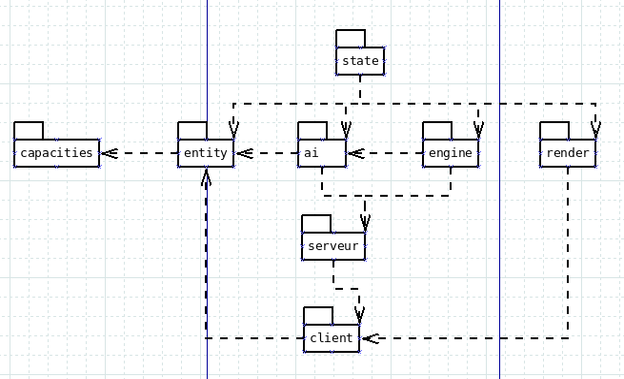
\includegraphics[width=0.80\textwidth]{lol.jpg}
\end{figure}
\end{document}
